\documentclass[UTF8, twoside]{EPURapport}
\usepackage{algpseudocode}
\usepackage{algorithm}
\usepackage{pdfpages}
\usepackage[nottoc, notlof, notlot]{tocbibind}
\usepackage{amsmath,amsfonts,amsthm}
\usepackage{graphicx}
\usepackage{rotating}
\usepackage{color}
\usepackage{colortbl}
%\usepackage{listings}

%\renewcommand{\lstlistlistingname}{Liste des codes}
%\renewcommand{\lstlistingname}{Code}

%\addextratables{%
%	\lstlistoflistings
%}

%\swapAuthorsAndSupervisors



\thedocument{Operational research project draft}{Ant colony optimization algorithm for a combined routing and scheduling problem}{Ant colony optimization algorithm for a combined routing and scheduling problem}

\grade{Computer Aided Decision Support\\ International Research Master 2\\ 2013 - 2014}

\authors{%
	\category{Student}{%
		\name{Thomas NOGUER} \mail{thomas.noguer@etu.univ-tours.fr}
	}
	\details{M2RI CADS 2013 - 2014}
}

\supervisors{%
	\category{Supervisors}{%
		\name{Jean-Charles BILLAUT} \mail{jean-charles.billaut@univ-tours.fr}
		\name{Nicolas MONMARCHÉ} \mail{nicolas.monmarche@univ-tours.fr}
	}
	\details{Université François-Rabelais, Tours}
}

\abstracts{abstract}
{keywords}

\begin{document}

\chapter{Formalization of the problem}

	The problem can be defined from three differents subproblems :
	
\begin{itemize}
\item[$\bullet$] The two machines permutation flowshop. We have two machines $M_1$ and $M_2$ organized as a flowshop. A set of $n$ jobs have to be scheduled into a sequence. Each job $j$ has a value $a_j$ and $b_j$ that correspond to the time required to complete the job $j$ on $M_1$ and $M_2$ respectively.
\item[$\bullet$] The grouping of jobs to be delivered. When the jobs are completed for the two machines permutation flowshop we must form groups of jobs, where a group must contain at least one job. These groups are then used for the third subproblem.
\item[$\bullet$] A traveling salesman problem. We consider one truck taking the group of jobs previously formed where each job has a destination $k_j$. The idea is to find the sequence of destinations in order to deliver every job from the group while minimizing the traveling distance. We have a matrix $K$ ($m \times m$) where $m$ is the number of destinations and $K_i^j$ is the distance between the destination $i$ and $j$.
\end{itemize}

	The objective function is to minimize the sum of lateness of the jobs $\sum_{j=1}^{j \leq n} L_j$. The lateness $L_j$  of a job $j$ is the difference between the completion time of the job $c_j$ and its due date $d_j$: $L_j = c_j - d_j$. The completion time of a job is not equal to the completion time of the job for the flowshop problem but for the traveling salesman problem. \textbf{$c_j$ is equal to the date at which the truck is coming back to the factory after its deliveries.}
\textbf{We consider that the truck has no capacity limit, it can carry has many jobs has possible.}
\\

	The input data of our problem are the following :
\begin{itemize}
\item[$\bullet$] The number $n$ of jobs,
\item[$\bullet$] The values $a_j$, $b_j$ and $d_j$ of job $j$ ($\forall j \in [1,n]$),
\item[$\bullet$] The number of $m$ destinations,
\item[$\bullet$] The destination $k_j$ of job $j$ ($\forall j \in [1,n]$),
\item[$\bullet$] The matrix $K$ ($m \times m$) of distances between each destination.\\
\end{itemize}

	During the resolution of the problem we must find the sequence of jobs on the flowshop, the groups of jobs to be delivered and the sequence of delivery for each group.

	We proposed a first way of encoding a solution : a table of size $n$ containing the sequence of job for the flowshop subproblem, a table of size $2n$ containing the groups and sequences for the traveling salesman subproblem. The first cell of the second table contains the number of jobs for the first group, the following cells contain the number of jobs in the delivery sequence and so on.
	
\begin{figure}
	\centering 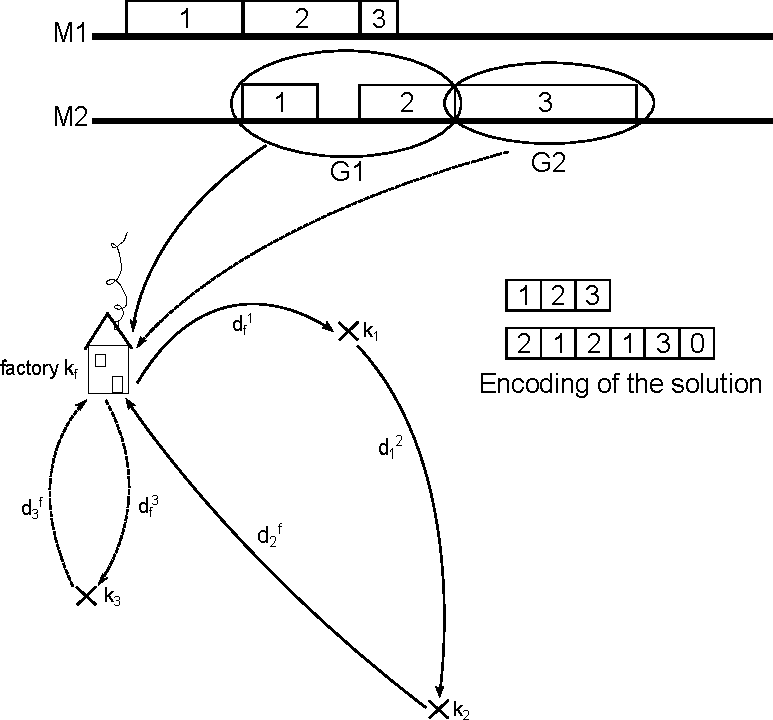
\includegraphics{images/problem.pdf}
	\caption {Schema of the problem}	
	\label {problem}
\end{figure}

\end{document}
